\documentclass[10pt]{article}
\usepackage{fontspec}
\setmainfont[AutoFakeSlant=0.2]{Noto Serif CJK SC}
\setsansfont{Noto Sans CJK SC}
\XeTeXlinebreaklocale "zh"
\XeTeXlinebreakskip=0pt plus 1pt
\renewcommand{\abstractname}{摘要}
\renewcommand{\figurename}{图}
\renewcommand{\tablename}{表}
\renewcommand{\refname}{参考文献}
\usepackage[a4paper,margin=21mm]{geometry}
\usepackage{amsmath,amssymb,booktabs,graphicx,url}
\usepackage[section]{placeins}
\usepackage[hidelinks]{hyperref}
\usepackage[numbers,sort&compress]{natbib}
\setlength{\emergencystretch}{2em}
\graphicspath{{../../../results/figures/}}
\newcommand{\RXXIIIReservedTasks}{96}
\newcommand{\RXXIIISpecs}{71}
\newcommand{\RXXIIIDetectable}{64}
\newcommand{\RXXIIILift}{44.39\%}
\newcommand{\RXXIIIP}{1.65e-19}
\newcommand{\RXXIVReservedTasks}{68}
\newcommand{\RXXIVSpecs}{141}
\newcommand{\RXXIVDetectable}{115}
\newcommand{\RXXIVReplays}{306}
\newcommand{\RXXIVLift}{44.33\%}
\newcommand{\RXXIVP}{8.29e-35}
\newcommand{\PublicRepoCount}{3}
\newcommand{\PublicMainlineCommits}{265}
\newcommand{\PublicModifiedSkills}{4058}


\title{从技能级到谓词级：面向演化型 LLM Agent 技能的预算化回归测试选择}
\author{匿名作者}
\date{匿名稿件，2026年9月}

\begin{document}
\maketitle

\begin{abstract}
可复用技能使语言模型 Agent 无需更新基础模型权重即可持久化操作流程，但每次技能修订都会产生回归测试问题。原生交互测试可能调用模型、模拟器或外部服务，重跑与被修改技能关联的全部案例会延迟反馈。本文研究能否把变更影响进一步定位到技能内部。PredicateImpact 将结构化技能变更映射为对象绑定、目标位置、设备或聚焦对象等动作谓词，再优先选择历史成功轨迹中覆盖该谓词的任务。方法先在已经暴露的 ALFWorld 与 ScienceWorld 任务上开发，再使用两份互不重叠、按内容盲规则抽取的名单评测。首次确认中，3任务预算内检出全部64个可检出谓词删除变更；技能家族随机的条件期望为55.61\%，绝对提升44.39个百分点，单侧精确检验 $p=1.65\times10^{-19}$。第二份名单同时检验删除、同类参数替换和相邻动作换序：115个可检出变更全部检出，强基线期望为55.67\%，提升44.33个百分点，$p=8.29\times10^{-35}$。三类算子和两个环境分别通过冻结门槛；491次原生回放的初始状态全部精确匹配，技术失败为0。候选与“在同一精确谓词覆盖集合内随机排序”完全持平，说明收益来自覆盖粒度，而不是复杂排序。事后噪声分析表明，即使漏记50\%真实覆盖边并误记20\%非覆盖边，平均提升仍为正。三个固定公开 Agent Skill 仓库的历史审计说明删除、替换和移动形态确实存在，但不能替代真实缺陷提交实验。因此，本文结论限于公开变异基准上的预算化检出，真实生产更新的总体外推仍待验证。
\end{abstract}

\noindent\textbf{关键词：}LLM Agent；Agent Skill；回归测试选择；变更影响分析；动态覆盖；变异测试

\section{引言}
Agent Skill 是持久化的流程、指令、脚本和资源，可在不改变基础模型权重的情况下扩展语言模型 Agent。近期系统已经能够从轨迹获取技能、持续修订、跨任务组合，并在共享技能库中执行准入治理\citep{ye2026mce,lei2026skillevolbench,gao2026skillaudit,song2026skillops}。这种持久性也带来了典型的软件维护义务：技能发生变化后，原来通过的行为必须重新验证。与普通单元测试不同，交互式 Agent 测试可能启动大模型、模拟器、外部服务或长链工具调用，因此立即全量回放可能代价很高。

最接近的 Agent Skill 系统已经注意到该问题。SkillAudit 在接纳或回滚更新前比较配对轨迹\citep{gao2026skillaudit}；SkillOps 表示技能契约与验证状态\citep{song2026skillops}；SkillFuzz 在查询预算下搜索技能组合\citep{hu2026skillfuzz}。FRAMES 与本文关系最直接：它先抽取与本轮被修改技能相关联的历史案例，再补充分层随机案例\citep{wang2026frames}。因此，“先测试被修改技能”本身不是新贡献。尚未解决的粒度问题是：当一次修订只改变一个条件、对象绑定、目标位置或工具步骤时，同一技能关联的全部案例是否仍应被等概率抽取。

传统回归测试选择通过程序变更与历史测试覆盖之间的联系处理类似问题\citep{rothermel1996rts}。但把该思想应用到 Agent Skill 并不直接：技能经常是自然语言而不是源码模块；轨迹包含别名和环境特定动作；语法变化不必然导致行为变化；测试结果昂贵且可能不稳定。评测还必须避免一个常见捷径，即在同一批任务上反复调整选择器，再把最终结果包装为显著性证据。

本文围绕一个结构化动作谓词层定义预算化 Agent Skill 回归测试。成功轨迹被映射为 \path{take_object=apple}、\path{place_destination=drawer} 或 \path{focus_object=thermometer} 等谓词。给定父子技能间定位到某一谓词的变更，PredicateImpact 先执行曾经覆盖该谓词的任务，再执行同技能家族的其他任务。这是一种轻量动态变更影响分析，不需要模型训练，并可直接使用发布门禁已经生成的轨迹。

研究完整保留了失败路径。早期粗粒度操作变异在同一技能家族中十分密集，精确操作覆盖相对技能家族随机几乎没有收益，甚至更差。只有在已暴露开发数据上写死稀疏谓词生成规则后，我们才进入谓词级研究；随后把规则和选择器原样应用到第一份内容盲名单。该确认通过后，又在打开第二份互斥名单前冻结“算子迁移”问题、三类算子和全部门槛。

本文贡献包括：
\begin{itemize}
  \item 提出面向固定交互预算的 Agent Skill 谓词级动态变更影响测试选择；
  \item 构建可审计的 ALFWorld/ScienceWorld 原生变异基准，包含结果盲开发、两份互斥内容盲名单、精确初始状态检查和输入哈希；
  \item 证明相对 FRAMES 式技能家族基线，谓词覆盖在两次确认中均把可检出变更的检出率提高约44个百分点，同时用强消融确定收益来自覆盖粒度而非排序；
  \item 给出三类算子、覆盖噪声网格、公开 \texttt{SKILL.md} 历史和家族密集负结果等外部有效性边界。
\end{itemize}

本文回答三个问题：\textbf{RQ1} 谓词级覆盖能否相对技能级关联提高早期检出？\textbf{RQ2} 该效果能否从动作删除迁移到参数替换和顺序变化，并同时出现在两个环境？\textbf{RQ3} 哪个方法组件产生收益，对不完整或错误的历史覆盖有多敏感？证据单位是冻结变异规格，而不是大模型家族或生产提交。

\section{相关工作}
\paragraph{技能演化与治理。}
Meta Context Engineering、AlignEvoSkill、SkillHone、SkillEvolBench 和 ContinualSkillBench 分别研究技能获取、改进、持久决策历史和长期评测\citep{ye2026mce,wang2025alignevoskill,li2026skillhone,lei2026skillevolbench,guan2026continualskillbench}。SkillCAT 结合对比证据和拓扑感知合并，SkillAudit 使用配对执行证据拒绝或回滚有害更新\citep{chen2026skillcat,gao2026skillaudit}。SkillOps 把技能库建模为带类型契约和验证状态的软件生态\citep{song2026skillops}。这些研究说明持续回归证据的重要性，但与同一技能绑定的测试并不一定具有同等信息量。

FRAMES 是最接近的测试策略基线。它优先处理与本轮修改技能关联的历史案例，再补充分层随机案例\citep{wang2026frames}。本文的技能家族随机基线获得同样的已修改技能信息；PredicateImpact 进一步考察家族内部的历史动态覆盖能否定位更小的影响集。SkillFuzz 使用抽取契约和差分预言机搜索组合中的隐含意图\citep{hu2026skillfuzz}，其测试单元、威胁模型和执行前阶段与更新后回归选择不同。

\paragraph{回归测试选择。}
回归测试选择从既有测试套件中挑选与修改程序相关的测试；经典评价维度包括包容性、精确性、效率和安全性\citep{rothermel1996rts}。动态方法记录通过测试执行了哪些程序实体，再重跑覆盖变化实体的测试。PredicateImpact 把这一设计迁移到 Agent Skill 的流程层，把动作谓词而不是源码语句或方法作为覆盖实体。本文不把经典 RTS 概念主张为原创，贡献在于面向演化技能的操作化和受控评测。

\paragraph{变异测试与交互基准。}
ALFWorld 把文本交互与具身家务任务对齐，ScienceWorld 提供程序生成的科学任务和 gold 动作序列\citep{shridhar2021alfworld,wang2022scienceworld}。当真实失败修订稀缺时，变异测试提供可控缺陷；但它可能偏向覆盖方法，因此必须加入多算子、未杀死变异、强基线和真实变更审计。本文固定 Anthropic、OpenAI、Microsoft 的公开 Agent Skill 仓库，只检查相应编辑形态是否出现\citep{anthropicskills2026,openaiskills2026,microsoftskills2026}，并不把其中的正常编辑标记为缺陷。

\section{问题定义}
令 $T=\{t_1,\ldots,t_n\}$ 为历史测试集合。任务 $t_i$ 属于技能家族 $g_i$，具有先前通过的动作轨迹 $\tau_i=(a_{i1},\ldots,a_{im})$ 和观测执行成本 $c_i$。确定性解析器 $\phi$ 把动作映射为谓词 $p=(k,v)$ 或空值。动态覆盖矩阵为
\begin{equation}
C_{ip}=\mathbb{1}\left[\exists a\in\tau_i:\phi(a)=p\right].
\end{equation}
结构化更新描述为 $\delta=(g,p)$，即技能家族 $g$ 在谓词 $p$ 处发生变化。实际系统可从类型化技能差分、作者标注或结构化流程解析器获得 $\delta$。本文假定该描述可用，不研究任意自然语言的自动定位。

更新后的技能在 $t_i$ 上产生二元失败指示 $Y_i(\delta)$。若 $\max_iY_i(\delta)=1$，则称该变更可被现有套件检出。预算为 $B$ 时，选择器返回有序子集 $S_B(\delta)$，其检出结果为
\begin{equation}
D_B(\delta)=\mathbb{1}\left[\max_{t_i\in S_B(\delta)}Y_i(\delta)=1\right].
\end{equation}
主要终点是可检出变更上的平均 $D_3$。同时报告保留全部未杀死变更的总变异得分。未杀死变更可能行为等价，也可能暴露测试套件不足，不能被重新标记为检出。

主要对照是技能级关联：已知 $g$ 后，从家族中均匀抽取 $B$ 个案例。若固定家族含 $N$ 个任务、其中 $K$ 个失败，其精确检出概率为
\begin{equation}
q(N,K,B)=1-\frac{\binom{N-K}{\min(B,N)}}{\binom{N}{\min(B,N)}}.
\end{equation}
该基线已知变化技能，因此强于全局随机。

\section{PredicateImpact 方法}
\subsection{谓词抽取}
固定解析器识别九类谓词。ScienceWorld 包含聚焦对象、启动设备、拾取对象和颜色箱目标；ALFWorld 包含拿取对象、放置目标、处理设备、打开目标和使用设备。解析过程规范化数字实例后缀和 inventory 别名。它规模小、可检查，不使用大模型或结果标签构建覆盖。

\begin{table}[t]
\centering
\caption{用于历史动态覆盖的固定动作谓词。}
\label{tab:predicateszh}
\begin{tabular}{lll}
\toprule
环境 & 谓词类型 & 示例值 \\
\midrule
ALFWorld & 拿取对象 & apple \\
ALFWorld & 放置目标 & drawer \\
ALFWorld & 处理设备 & sink basin \\
ALFWorld & 打开目标/使用设备 & safe / desk lamp \\
ScienceWorld & 聚焦对象 & thermometer \\
ScienceWorld & 启动设备 & thermometer \\
ScienceWorld & 拾取对象 & wire \\
ScienceWorld & 颜色箱目标 & blue box \\
\bottomrule
\end{tabular}
\end{table}

\subsection{选择规则}
PredicateImpact 首先排列修改家族中覆盖 $p$ 的任务，然后是同家族未覆盖任务，最后是其他家族。覆盖集合内部优先选择匹配点之后剩余轨迹比例更大、每次匹配对应健康步数更少的任务。若首个匹配位置为 $j_i$，轨迹长度为 $m_i$，其优先项为
\begin{equation}
r_i=\left(-\frac{m_i-j_i}{m_i},\frac{c_i}{\#\{a\in\tau_i:\phi(a)=p\}}\right).
\end{equation}
稳定任务标识用于最终打破平局。预算增加时仍可继续执行完整测试集，因此该方法改变顺序而不永久删除证据。

实现需要线性扫描历史轨迹并排序。更重要的是，实验加入“谓词覆盖集合内随机”消融：它得到完全相同的覆盖任务集合，只随机化内部顺序。若该消融与候选持平，可辩护的贡献就是覆盖粒度，而不是 $r_i$。

\subsection{对照方法}
对照包括：谓词覆盖集合内随机、作为主基线的技能家族随机、全局随机、家族分层随机、更新描述与任务目标的词汇相似、最短健康测试优先，以及读取结果的预言机上界。随机方法使用200个稳定种子。只有技能家族随机进入冻结主提升和条件随机化检验；覆盖集合随机用于诊断收益来源。

\section{实验设计}
\subsection{开发与暴露控制}
开发集包含此前已暴露的78个 ScienceWorld 和30个 ALFWorld 任务，其中分别有71和27条成功健康参考。在读取任何变异结果之前，固定生成器只保留同家族覆盖数至少1且不超过成功任务一半的谓词；每个“家族×谓词类型”最多保留1个单任务谓词和4个多任务谓词。第一份从未执行的草案因96个规格中74个是单任务谓词而被否决并保留，避免静默改写协议。最终开发集含77个规格，其中72个可检出。

晋级条件预先要求至少30个可检出规格、10个多任务规格、2个环境和8个技能家族；检出率至少0.80，相对技能家族随机绝对提升至少0.20，单侧条件 $p\leq0.01$。开发结果通过后，算法和首次确认协议被冻结。

\subsection{第一次独立确认}
暴露账本先识别已经出现在项目文件中的任务引用。在读取目标、gold路径或结果之前，SHA-256排序从ALFWorld六个家族各取8个 \texttt{valid\_unseen} 案例，并从ScienceWorld三个家族各取16个官方测试变体，共96个。健康参考使用ALFWorld手工专家或ScienceWorld gold序列。5个ALFWorld双对象参考在固定步数内失败并完整保留，剩余91个成功参考参与覆盖。

开发生成器原样产生\RXXIIISpecs{}个删除规格和185次原生回放。首次确认重复开发门槛，并额外要求每个环境检出率至少0.75、提升至少0.15、单侧 $p\leq0.05$。打开名单后不允许修改阈值。

\subsection{算子迁移确认}
R24在观察R23之后设计，因此它是新的确认问题，不是整个研究流程的预注册复制。但在打开第二份名单内容之前，代码、三类算子、抽样、终点和门槛全部冻结。名单包含R23之后剩余的32个兼容ALFWorld任务，以及ScienceWorld每个家族12个未使用测试变体，共68个任务，与R23重叠为0，68条健康参考全部成功。

基础谓词在适用时扩为三类算子：
\begin{enumerate}
  \item \textbf{删除：}移除首次匹配动作；
  \item \textbf{参数替换：}用历史上可执行、谓词类型相同但参数不同的动作替换；
  \item \textbf{相邻换序：}交换匹配动作与其后一动作。
\end{enumerate}
适用性仅从健康轨迹推导。冻结产物包含141个算子规格和306次计划原生回放。总体门槛要求至少30个可检出规格、3类算子、2个环境和6个家族；检出率至少0.75、提升至少0.15、$p\leq0.01$。每类算子还须至少6个可检出规格、检出率至少0.65、提升至少0.10。

\subsection{原生执行与审计}
每条变异轨迹都从全新环境重置开始执行。初始观察、目标和可行动作集合的哈希必须与健康参考一致。环境异常记为技术错误，绝不计作杀死变异。ScienceWorld 使用固定上游模拟器 JAR，任务划分成员关系在采集时检查。实验运行在AMD EPYC~7642宿主上，容器配额为20核CPU、90~GiB内存；机器带RTX~3090，但确认实验不执行模型推理，因此未使用GPU。164条独立名单健康参考和491次变异回放的逐episode耗时合计约22.1分钟。

每个运行规格对代码、配置、名单、模拟器、健康轨迹和上游实现计算哈希。审计器把路径限制在项目根目录内，检查全部输入哈希、原实现源码和任务名单。两次确认的491次回放全部精确匹配初始状态，技术失败为0。

\subsection{统计范围}
对每个可检出规格，使用上式精确计算家族随机检出概率。各规格独立随机选择产生 Poisson--binomial 零假设分布，报告 PredicateImpact 实际检出数对应的单侧上尾概率。该检验只比较冻结基准上的随机选择机制，不是未来技能、任务家族、仓库或算子总体推断。两个环境和三类算子分别报告，冻结门槛防止事后挑选有利子组。

\section{实验结果}
\subsection{RQ1：谓词覆盖提高早期检出}
表\ref{tab:mainzh}给出两次确认。PredicateImpact在3任务内检出全部可检出规格。R23检出率为1.000，技能家族随机期望为0.5561，绝对提升\RXXIIILift{}（$p=1.65\times10^{-19}$）。ALFWorld提升0.3565（$p=5.29\times10^{-7}$），ScienceWorld提升0.5164（$p=3.12\times10^{-13}$），10项冻结确认条件全部通过。

把7个没有被任何任务杀死的规格也计入后，候选R23总变异得分为0.9014，技能家族随机期望为0.5012。相对重跑修改家族中的全部合格任务，每个可检出更新至多执行3个任务使执行数减少75.45\%。

\begin{table}[t]
\centering
\caption{3任务预算下的独立确认。主检出率以现有套件可检出变更为条件；总变异得分保留所有未杀死变更。}
\label{tab:mainzh}
\resizebox{\linewidth}{!}{%
\begin{tabular}{lrrrrrrrr}
\toprule
实验 & 任务 & 规格 & 可检出 & 谓词方法 & 家族随机 & 提升 & 总变异得分 & 执行减少 \\
\midrule
R23删除确认 & 96 & 71 & 64 & 1.0000 & 0.5561 & 0.4439 & 0.9014 & 0.7545 \\
R24三算子 & 68 & 141 & 115 & 1.0000 & 0.5567 & 0.4433 & 0.8156 & 0.7132 \\
\bottomrule
\end{tabular}}
\end{table}

\begin{figure}[t]
\centering
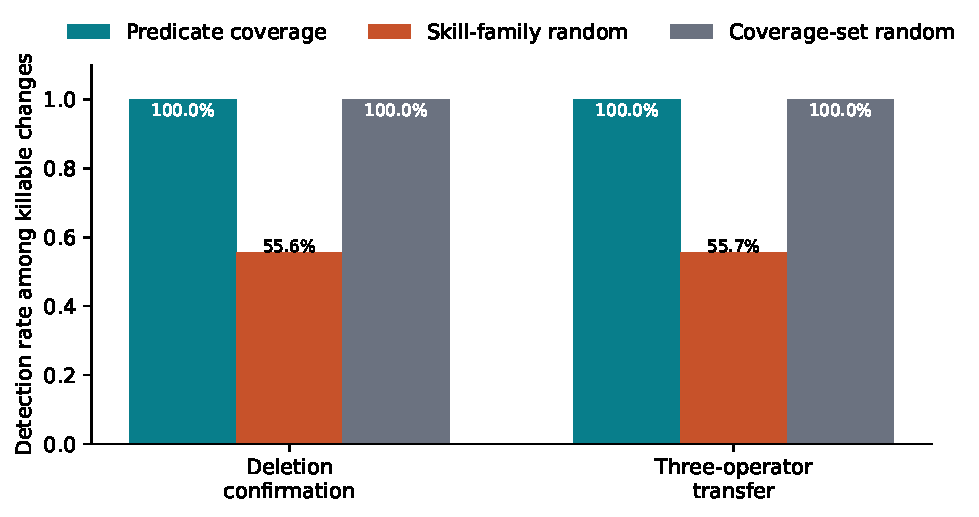
\includegraphics[width=.85\linewidth]{predicate_confirmation.pdf}
\caption{可检出变更上的检出率。PredicateImpact与精确谓词覆盖集合内随机持平，二者均优于技能家族随机。}
\label{fig:confirmationzh}
\end{figure}

\subsection{RQ2：结果跨算子和环境迁移}
互斥R24名单给出几乎相同的总体结果：检出率1.000，技能家族随机期望0.5567，提升\RXXIVLift{}，$p=8.29\times10^{-35}$。ALFWorld与ScienceWorld提升分别为0.3595和0.5346。表\ref{tab:operatorszh}显示删除、同类参数替换和相邻动作换序分别越过事先门槛。最小的换序层只有18个可检出变更，但提升仍为0.4038，条件 $p=1.16\times10^{-5}$。10项算子迁移门槛全部通过。

141个R24规格中有26个未被任何任务杀死。保留它们后，PredicateImpact总变异得分为0.8156，技能家族随机期望为0.4541。由于现有测试套件不能证明语义等价，本文不把这些存活项直接称为等价变异。

\begin{table}[t]
\centering
\caption{R24按变异算子分层的结果。}
\label{tab:operatorszh}
\begin{tabular}{lrrrr}
\toprule
算子 & 可检出数 & 谓词方法 & 家族随机 & 提升 \\
\midrule
删除匹配动作 & 58 & 1.0000 & 0.5745 & 0.4255 \\
同类参数替换 & 39 & 1.0000 & 0.5120 & 0.4880 \\
相邻动作换序 & 18 & 1.0000 & 0.5962 & 0.4038 \\
\bottomrule
\end{tabular}
\end{table}

\subsection{RQ3：覆盖粒度解释收益}
精确谓词覆盖集合内随机在两次确认中同样检出全部可检出变更（图\ref{fig:confirmationzh}）。因此，PredicateImpact的下游跨度与成本平局规则在主预算下没有观测到额外提升。词汇相似有时能从任务文字中恢复谓词值，但不能提供同样稳定的覆盖；最短优先与全局策略也常把早期预算用在真实影响集之外。结果支持更简单的系统设计：首先可靠记录谓词覆盖；只有在出现“多个覆盖任务具有不同失败传播”的数据后，复杂集合内排序才值得获得方法贡献。

早期负结果说明何时该信息无用。对粗粒度ScienceWorld操作变异，机会感知选择检出28个可检出“家族×算子”中的27个，但家族随机期望已达0.9016（提升0.0627，$p=0.119$）。ALFWorld中候选检出33个中的31个，而家族随机期望为0.9727（提升$-0.0333$，$p=0.984$）。若一个变更影响技能关联的几乎全部测试，技能级关联已经足够；谓词覆盖主要用于稀疏条件性变更。

\section{鲁棒性与外部依据}
\subsection{覆盖损坏}
R24出现部分日志、但尚未完成时，我们固定了一项事后敏感性网格；它不是确认性证据。真实覆盖边以0--0.50概率独立漏记，同家族非覆盖边以0--0.20概率误记。20种组合各使用500个稳定哈希种子，观测覆盖任务内部按健康执行成本排序。

漏记20\%、误记10\%时，R23和R24平均检出率分别为0.9478和0.9258，相对家族随机仍提升0.3918和0.3690。在最严重的50\%/20\%组合下，检出率为0.7695和0.7358，提升0.2134和0.1791；两个数据集的500次模拟均保持总体正提升。这些分位数描述指定的覆盖损坏机制，不是部署总体抽样不确定性。

\begin{figure}[t]
\centering
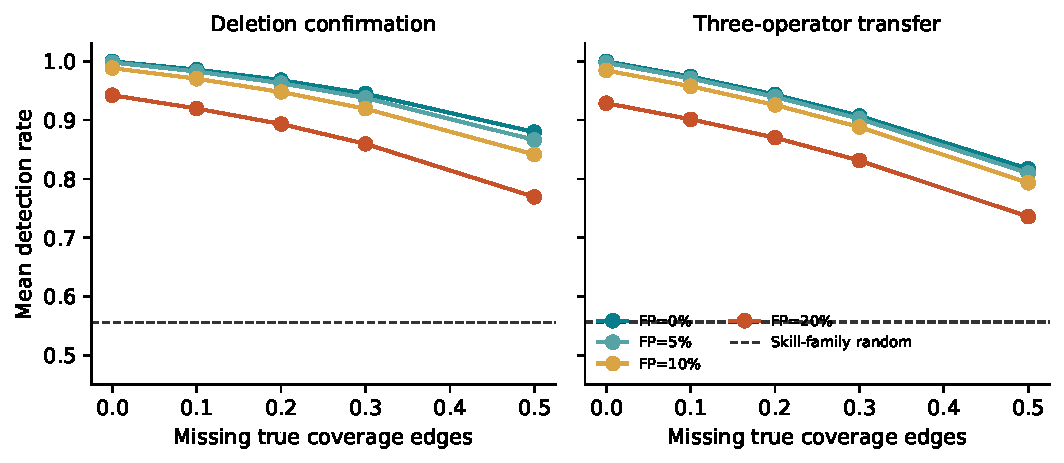
\includegraphics[width=\linewidth]{coverage_noise.pdf}
\caption{事后覆盖噪声敏感性。虚线为精确技能家族随机期望，FP表示误记边比例。}
\label{fig:noisezh}
\end{figure}

\subsection{公开Skill历史审计}
为检查三类算子是否完全人为，我们在R24算子固定后锁定Anthropic、OpenAI和Microsoft三个公开Agent Skill仓库的主分支\citep{anthropicskills2026,openaiskills2026,microsoftskills2026}，遍历265个一方主线提交。120个提交修改了既有 \texttt{SKILL.md}，对应4,058个文件修改；其中3,952个来自Microsoft批量文档同步，因此文件不能视为独立观测。

零上下文差分启发式发现：4,037个修改含删除，4,028个含混合增删hunk，3,835个存在相似行替换候选，665个存在相同行移动候选。三个仓库都出现删除、替换形态和移动形态。审计只发布提交ID、路径、计数和哈希，不复制第三方正文。这只能为结构编辑原语提供依据，不能说明公开编辑存在缺陷，也不能证明PredicateImpact会为它选中失败的生产测试。

\section{讨论}
\paragraph{实践含义。}
可操作结论很克制：已经记录成功任务轨迹的发布系统，不应只把轨迹绑定到整个技能，还应记录每个任务执行过哪些结构化条件、对象绑定、目标位置和工具步骤。当差分定位到某个谓词时，先回放覆盖任务，再从技能家族广泛抽样。在冻结基准中，该策略用至多3个原生测试检出所有可检出变更，并减少约71--75\%的全家族执行。

\paragraph{没有得到支持的结论。}
实验没有证明下游跨度排序优于同影响集随机，没有证明自由文本差分能自动定位，也没有证明任何语义后果都能被选中任务暴露，更没有证明3个测试足以安全发布。“检出”仅表示受控变异使至少一个现有任务失去成功终态。真实门禁仍应在高风险、新颖变更或覆盖不确定时扩展到更广的分层测试。

\paragraph{与失败恢复研究的关系。}
本项目最初尝试使用谱系和反事实重蒸馏修复受污染后代。受控模拟显示成本收益，但三个模型家族、288个原生模型--任务对没有产生稳定恢复提升。我们没有继续在同一测试结果上调整恢复器，而是改变生命周期问题：任意技能更新发生后，应先执行哪些测试？原负结果完整保留在产物中，不计作PredicateImpact的正证据。

\section{有效性威胁}
\paragraph{构念有效性。}
被变异的流程单元是记录下来的成功动作程序。许多生产Agent Skill是由LLM解释的自然语言文档，因此本文测量的是可插桩流程层的回归选择，而不是任意 \texttt{SKILL.md} 文本的端到端解释。专家和gold轨迹消除了执行器噪声，也降低了生态复杂度。

更新描述给出正确技能家族、谓词类型和值；现实差分定位可能含糊。噪声实验扰动覆盖边，但没有扰动变更描述。终态成功适合当前环境，真实系统还可能要求安全、延迟、成本或政策断言。

\paragraph{内部有效性。}
变异位置由历史覆盖产生，因此结构上有利于覆盖选择器。这是动态RTS的基本耦合假设，但若真实缺陷传播到未覆盖实体，效果可能被夸大。本文通过两份互斥名单、三类算子、存活变异报告、精确状态匹配和公开编辑形态审计缓解但不能消除该威胁。技术异常不计为杀死。

R24在R23之后设计，只确认算子迁移，不是完整研究流程的未接触复制。覆盖噪声网格是在部分R24日志可见后固定，明确属于事后分析。R23仍是R22规则的主要独立确认。

\paragraph{统计与外部有效性。}
条件随机化 $p$ 值说明在这些固定变更上，当前检出数相对指定家族随机机制有多意外，不表示从所有技能中随机抽样。基准只有两个文本环境，R23含9个家族、R24含8个，未覆盖Web、代码、多模态、多Agent和在线服务副作用。公开仓库修改高度聚类于仓库和同步提交。带独立失败测试的真实技能缺陷提交仍是最重要的缺失证据。

\section{可复现性}
产物按研究阶段隔离并保留全部失败前序。R22包含结果盲生成器和开发结果；R23、R24包含冻结名单、健康轨迹、变异规格、原始原生结果、选择器评价、完成记录和独立哈希审计；R25包含公开仓库固定信息和聚合差分记录；R26包含完整噪声网格及其时序警告。表图由 \texttt{analysis/regression\_submission.py} 重新生成。

核心确认需要Python、ALFWorld 0.4.2、TextWorld 1.7.0、ScienceWorld 1.2.3、固定模拟器JAR和OpenJDK 17；不需要Docker、GPU、模型权重或外部API。上游基准数据不随产物再分发，清单和环境脚本给出预期位置。内容哈希绑定全部本地输入，公开表格保留比正文更高的精度。

\section{结论}
演化型Agent Skill的预算化回归测试可以从技能内部信息获益。在两份互斥的ALFWorld/ScienceWorld名单上，3任务预算下的谓词级动态覆盖相对强技能家族随机基线把可检出变更检出率提高约44个百分点；该效果跨动作删除、同类参数替换和相邻换序重复出现。最强消融与候选持平，准确界定了贡献：细粒度影响覆盖有效，而集合内排序尚未获得证据。指定覆盖噪声下性能平稳下降，公开历史也存在相应编辑形态。走向生产证据的下一步，是在具有独立失败测试的自然技能缺陷提交上评测，并解决自由文本差分的自动定位。

\bibliographystyle{plainnat}
\bibliography{../../references}

\appendix
\section{冻结门槛汇总}
R23对可检出和多任务规格数、两个环境、八个家族、总体检出率/提升/$p$，以及每个环境的检出率/提升/$p$设定最低要求。R24对可检出规格数、三类算子、两个环境、六个家族、总体检出率/提升/$p$，以及每类算子的数量、检出率和提升设定要求。机器可读完成文件中全部检查均为真。

\section{证据分母}
R23含71个规格，其中64个可检出；R24含141个规格，其中115个可检出。主要终点以可检出为条件，因为现有套件中没有失败任务的变更不可能被任何选择器发现。总变异得分保留全部规格，以暴露这一条件化处理。衍生主张不得把“可检出变更检出率”改写为无条件的“缺陷检出率”。

\section{暴露时间线}
开发只使用早期恢复实验已暴露任务。R23在打开任务内容前根据标识层清单冻结名单。R24排除全部R23标识，先冻结代码和名单，再收集健康轨迹。R25公开仓库快照只在R24算子固定后选择。R26因写入噪声网格时已看到部分R24结果而明确标记为事后分析。

\end{document}
